Las estrellas de neutrones son sistemas astronómicos con nucleones sometidos a condiciones extremas.
Debido a la repulsión de Coulomb entre protones el sistema tiene inhomogeneidades en su estructura.
Estas inhomogeneidades aparecen también en sistemas expandiéndose, donde la distribución de fragmentos depende de las condiciones termodinámicas (temperatura, fracción de protones, \ldots) y la velocidad de expansión.

El objetivo es estudiar distintos regímenes de distribución de fragmentos y la existencia de clusters infinitos. Comenzando con una configuración de equilibrio, expandimos el sistema homogéneamente hasta llegar a una configuración asintótica (i.\ e.\ densidades finales muy bajas).
Estudiamos la distribución de fragmentos a lo largo de la expansión.

Encontramos los típicos regímenes de la distribución de fragmentos de una expansión: U-shaped, ley de potencias y exponencial.
Otra característica de nuestro cálculo es que, ya que la interacción entre protones es repulsiva de largo rango, no siempre tenemos un fragmento infinoto.
Como es de esperar, cuanto más rápida es la velocidad e expansión, más rápido desaparece el fragmento infinito.

Desarrollamos una herramienta basada en análisis de grafos para la identificación del fragmento infinito y encontramos una transición de distribución de fragmentos de U-shaped a exponencial a medida que aumenta la velocidad de expansión.

\section{Introducción}
\todo[inline]{Acá una pequeña introducción respecto de los analizadores de fragmentos utilizados y, probablemente, un apéndice}

\section{Fragmento infinito}

En la figura~\ref{fig:morpho} mostramos los estados inicial y final de la expansión de la celda principial de $N=11000$ partículas para velocidades de expansión muy bajas.
Podemos ver que, más allá de que la configuración inicial muestra una distribución de partículas compacta, la configuración final consiste de \emph{gnocchi} (casi esféricos) con una masa de alrededor de 80 partículas.

\begin{figure} \centering
  \begin{subfigure}[h!]{0.45\columnwidth}
    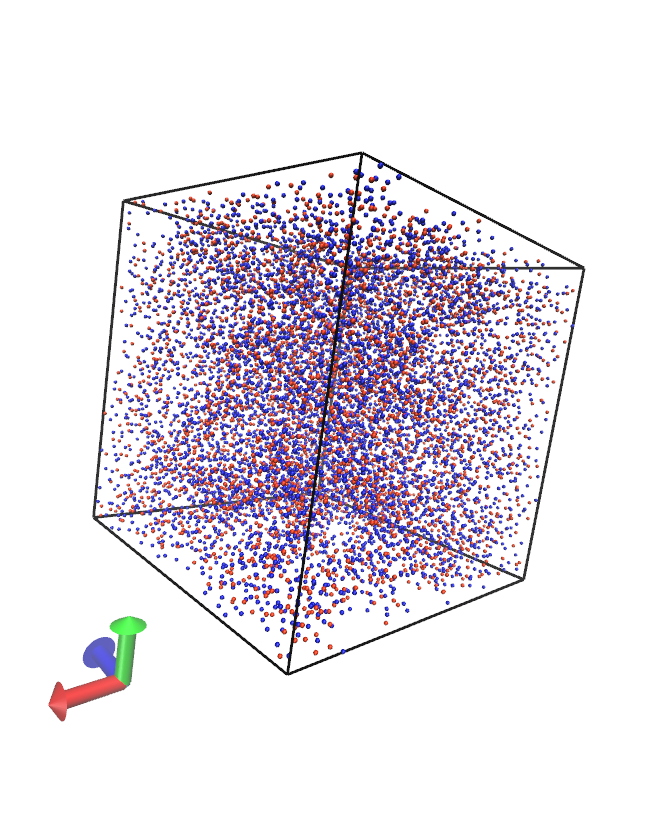
\includegraphics[width=\columnwidth]{fragmentacion/initial}
    \caption{$\eta = 0.0001\,\text{fm/c}$}
    \label{subfig:initial}
  \end{subfigure}
  \begin{subfigure}[h!]{0.45\columnwidth}
    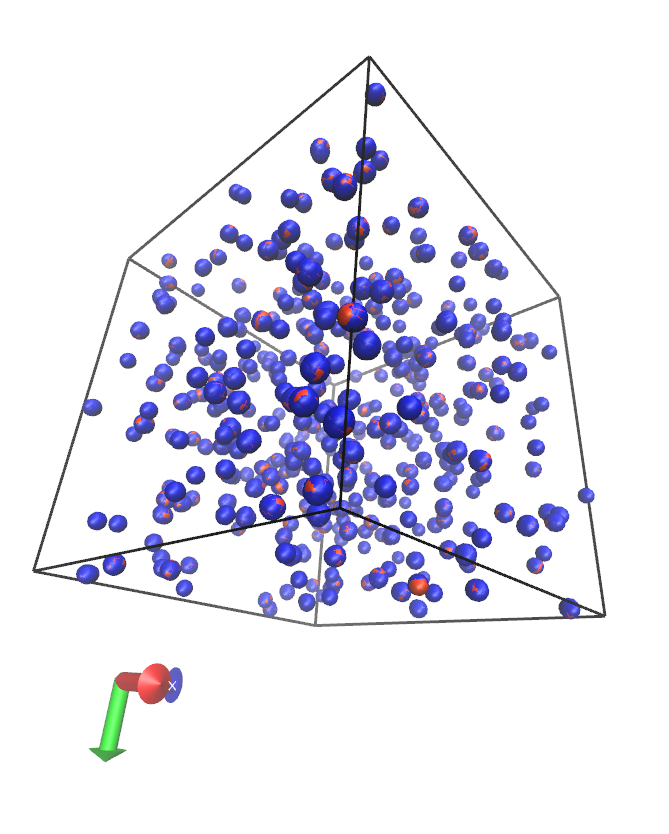
\includegraphics[width=\columnwidth]{fragmentacion/expanded}
    \caption{$\eta = 0.0005\,\text{fm/c}$}
    \label{subfig:expanded}
  \end{subfigure}
  \caption{Estructuras de un sistema en su configuración inicial~\ref{subfig:initial} y el sistema expandido final~\ref{subfig:expanded}.
    En el sistema expandido podemos ver que se forman fragmentos de tipo \emph{gnocchi}.}
  \label{fig:morpho}
\end{figure}

En la figura~\ref{fig:infinite} mostramos la fracción de partículas en la celda principal que forman parte de un cluster infinito (\emph{Fracción de Fragmento Infinito}, FFI).
Podemos ver fácilmente que en las primeras etapas de la evolución, como la temperatura es baja, la mayor parte del sistema en la celda principal pertenence al fragmento infinito.
Sin embargo, a medida que evoluciona el sistema de acuerdo a la velocidad de expansión, la FFI disminuye y llega a cero rápidamente, implicando que no hay fragmentos infinitos en el sistema.

\begin{figure}
  \centering
  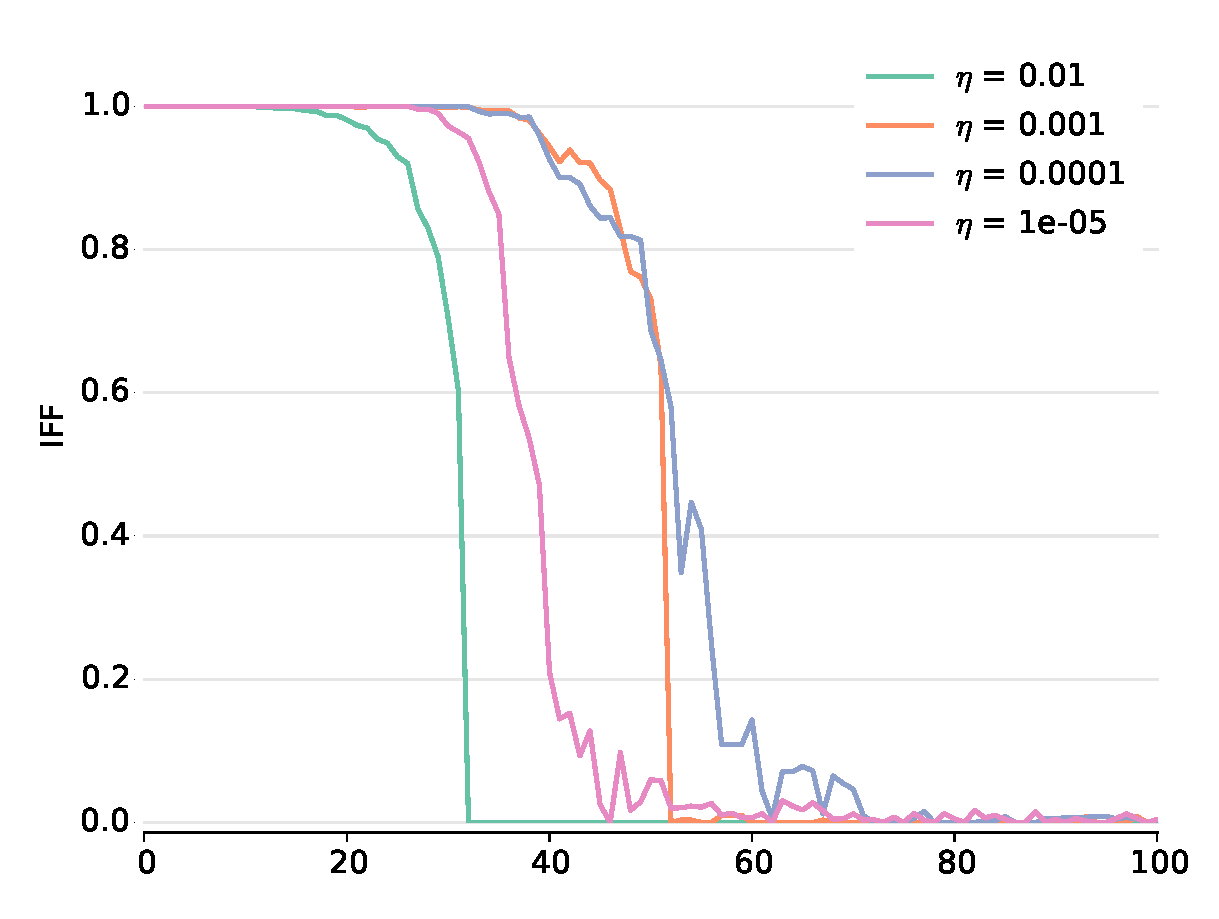
\includegraphics[width=0.75\columnwidth]{fragmentacion/infinite.pdf}
  \caption{Fracción de Fragmento Infinito (ver texto) en función de la longitud de la celda principal.
    Para todas las velocidades de expansión mostradas el FFI va a cero en el régimen asintótico.}
  \label{fig:infinite}
\end{figure}

\section{Fragmentos asintóticos}

La figura~\ref{fig:distribution} muestra la distribución de fragmentos asintóticos para cuatro distintas velocidades de expansión.
En este caso, el algoritmo MSTE fue aplicado sobre la celda principal, considerando las condiciones periódicas de contorno y sabiendo que no hay fragmento infinito, como se ve de la figura~\ref{fig:infinite}.
Podemos ver que a medida que aumenta la velocidad de expansión, la distribución de fragmentos muestra la típica transición de U-shaped a decaimiento exponencial.
Entre estas dos, aparece una distribución de tipo ley de potencias.
En particular, la figura~\ref{subfig:9e-3} muestra que con una expansión de $\eta = 0.009\,\text{fm/c}$ obtenemos una ley de potencias.
Es interesante notar que a diferencia de casos típicos de estudios de fragmentos, como percolación o sistemas de Lennard-Jones, debido a la presencia del término de repulsión de Coulomb, no es posible ver un fragmento infinito en el régimen asintótico.

\begin{figure} \centering
  \begin{subfigure}[h!]{0.45\columnwidth}
    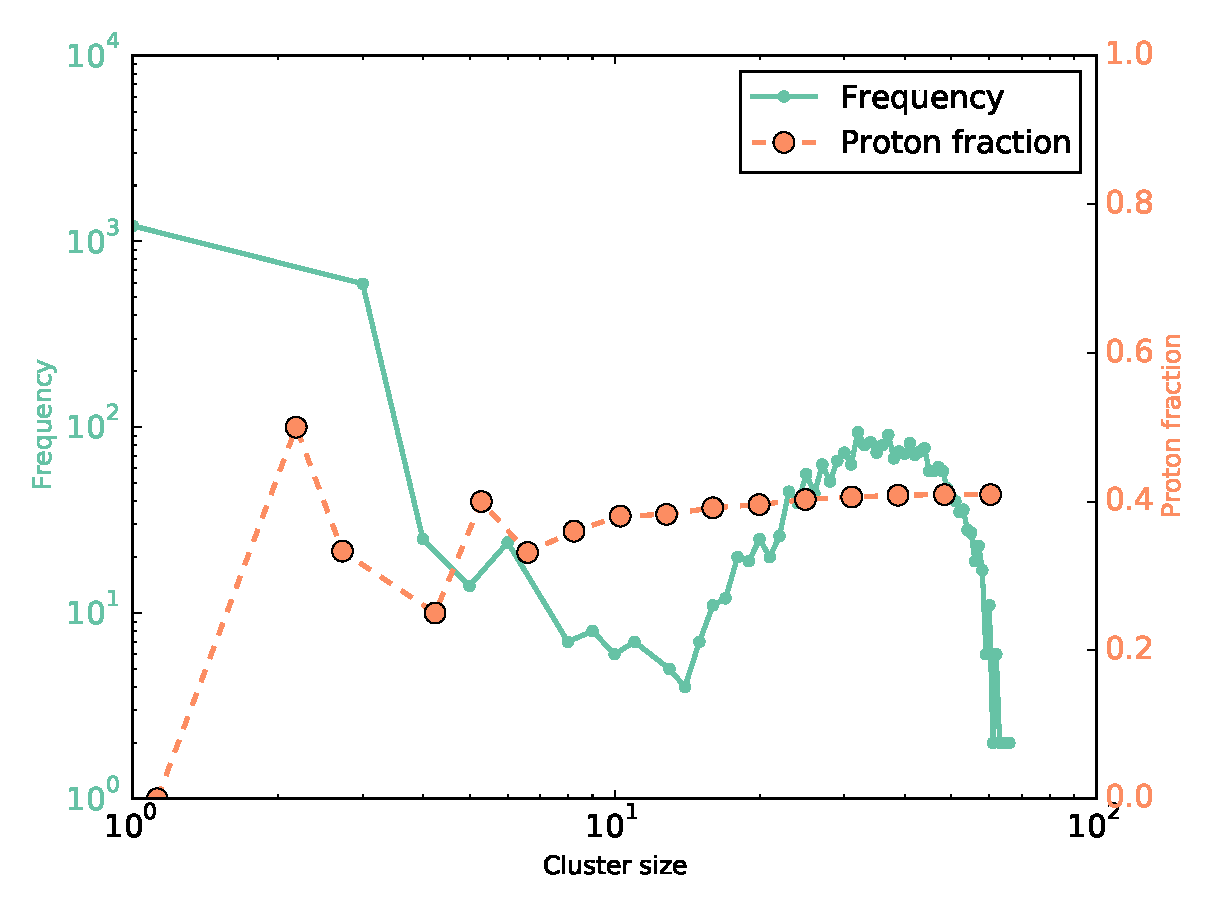
\includegraphics[width=\columnwidth]{fragmentacion/cluster_1e-4}
    \caption{$\eta = 0.0001\,\text{fm/c}$}
    \label{subfig:1e-4}
  \end{subfigure}
  \begin{subfigure}[h!]{0.45\columnwidth}
    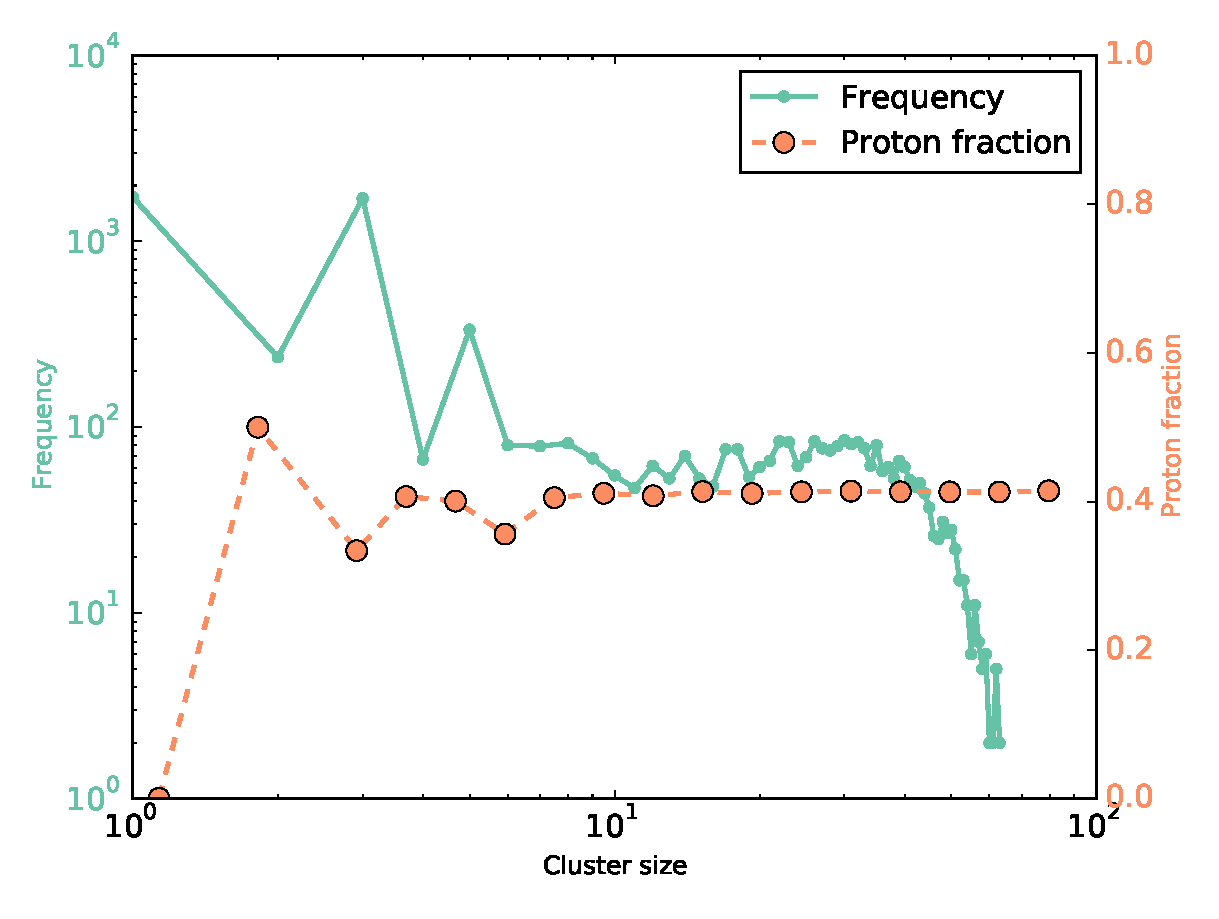
\includegraphics[width=\columnwidth]{fragmentacion/cluster_5e-4}
    \caption{$\eta = 0.0005\,\text{fm/c}$}
    \label{subfig:5e-4}
  \end{subfigure}
  \begin{subfigure}[h!]{0.45\columnwidth}
    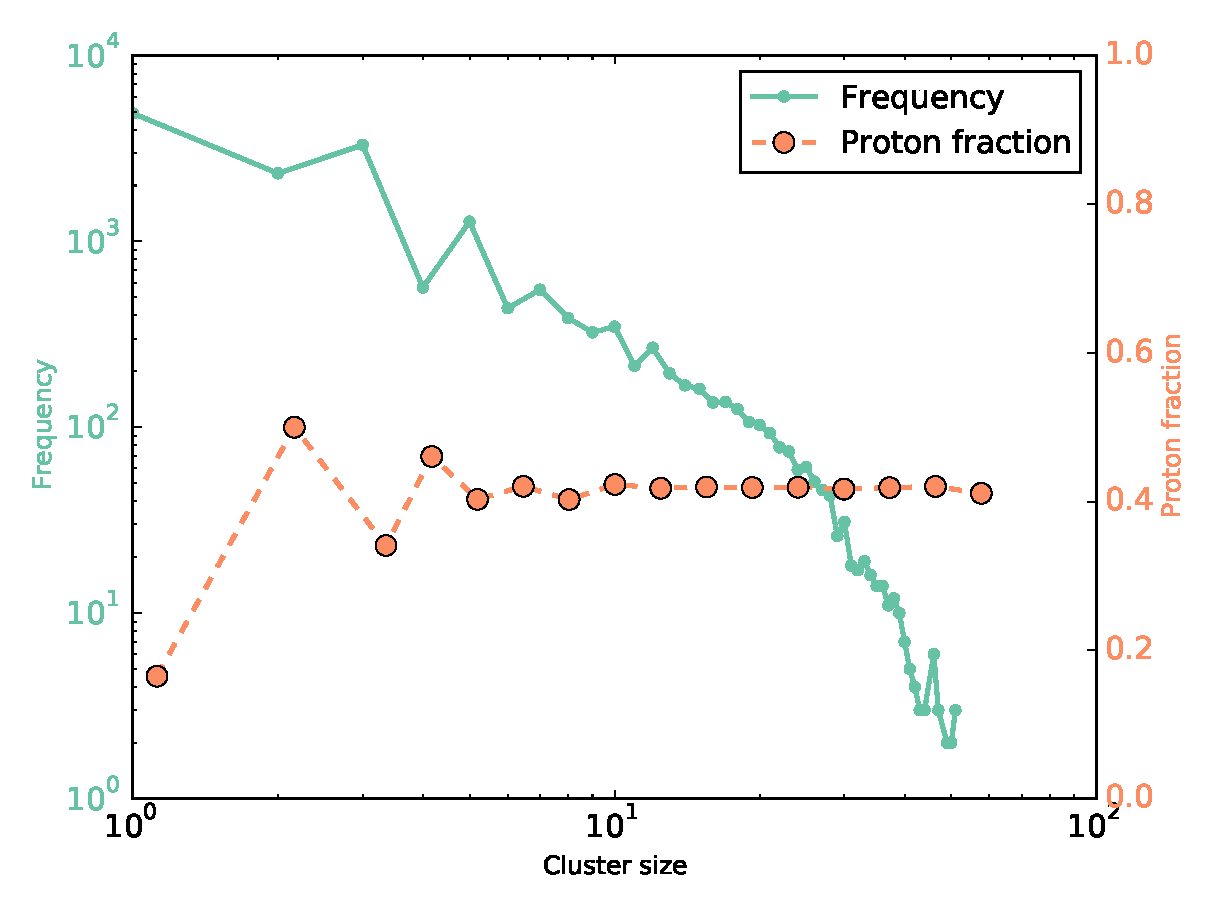
\includegraphics[width=\columnwidth]{fragmentacion/cluster_9e-3}
    \caption{$\eta = 0.009\,\text{fm/c}$}
    \label{subfig:9e-3}
  \end{subfigure}
  \begin{subfigure}[h!]{0.45\columnwidth}
    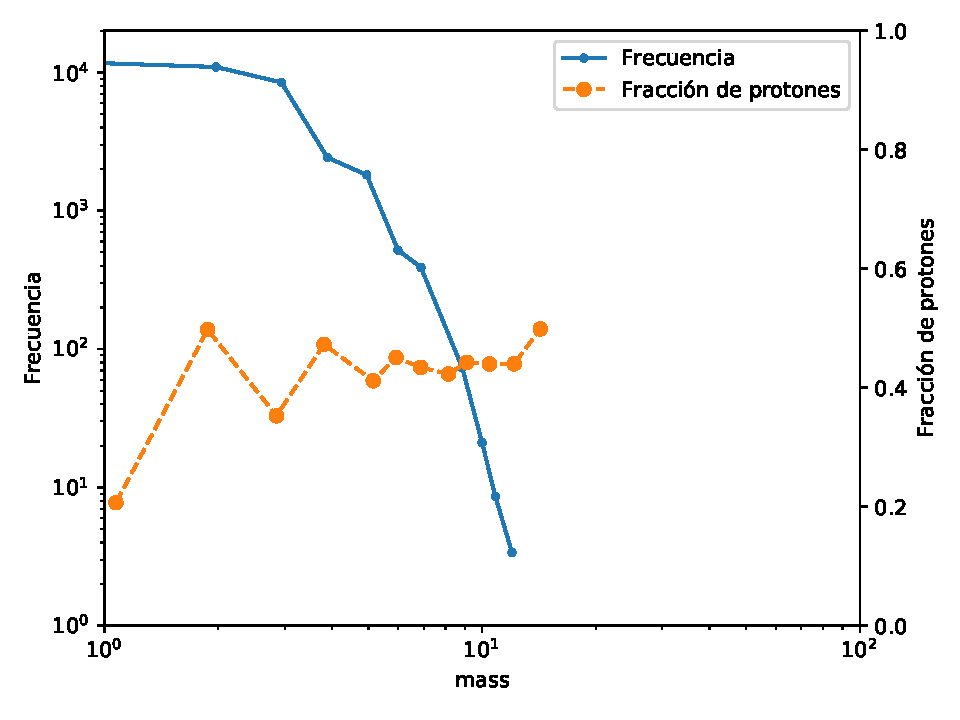
\includegraphics[width=\columnwidth]{fragmentacion/cluster_3e-2}
    \caption{$\eta = 0.03\,\text{fm/c}$}
    \label{subfig:3e-2}
  \end{subfigure}
  \caption{(Color online) Fragment mass distribution. Labels grow with larger
    expansion rates. System consisting of 11000 particles with
    $x=0.4$ and initial density $\rho_0 = 0.08\,\text{fm}^{-3}$}
  \label{fig:distribution}
\end{figure}

\section{Conclusiones}

Desarrollamos experimentos numéricos de sistemas expandidos homogéneamente  y, para analizar la estructura del sistema en función del tiempo, desarrollamos una herramienta basada en análisis de grafos para identificar fragmentos infinitos para cualquier tipo de fragmentos aditivios.
Una vez que esta formalismo fue aplicado a las simulaciones mencionadas, pudimos identificar la región en la que se da una distribución de fragmentos de tipo ley de potencias.
Esta distribución tiene formas desde U-shaped hasta decaimiento exponencial.
